\section{レーザー測定の方法と使用装置}
\subsection{レーザーの性能}
今回のLGAD検出器の増幅率の測定においては、図\ref{fg:Laser} の赤外線パルスレーザーを使用する。
このレーザーは、NKT Photonics社のKATANA 10 \cite{KATANA10}で、レーザーの性能について 表\ref{tab:Laser_performance} にまとめた。
このレーザーはトリガーを発行することができる。
レーザーのタイミングジッタは10 ps未満である、時間分解能に影響があると考える。
また、このレーザーの波長は1064 nmで、周波数を0.05から1 MHzに可変することができる。今回の測定では、周波数は1 MHzに設定した。

赤外線パルスレーザーから1秒間におよそ$5\times10^{16}$ 個の光子が出力されるため、1つの光子が落とすエネルギーは深さ方向にばらつきがあるが、
検出器内に入射する光子の数が非常に多いため、あたかもエネルギー損失が一様な粒子を模擬することができる。
そのため、ランダウノイズの効果が少ない状況で時間分解能を測定することができる。
また、レーザーの信号波形はほとんど同じであるため、タイムウォークの影響もほぼ無視できる。
そのため、この測定系で時間分解能を測定することで、ジッターのみの影響を評価することができる。
レーザーの波の向きは1つの方向に偏っているため、レーザー本体の上部にあるつまみを回すことで、偏向板減衰フィルターの角度を変えることで、レーザーの強度を調整することができる。
本実験では、PINの信号が小さいため、その信号がノイズに埋もれないようにレーザーの出力を最大にして測定を行なった。
レーザー装置内にあるハーフミラーで参照光の進む方向を、レーザーと同じ光軸上にすることができる。
その参照光を使って、レーザーの入射位置を知ることができる。

\begin{figure}[h]
    \begin{minipage}[c]{0.45\linewidth}
        \centering
        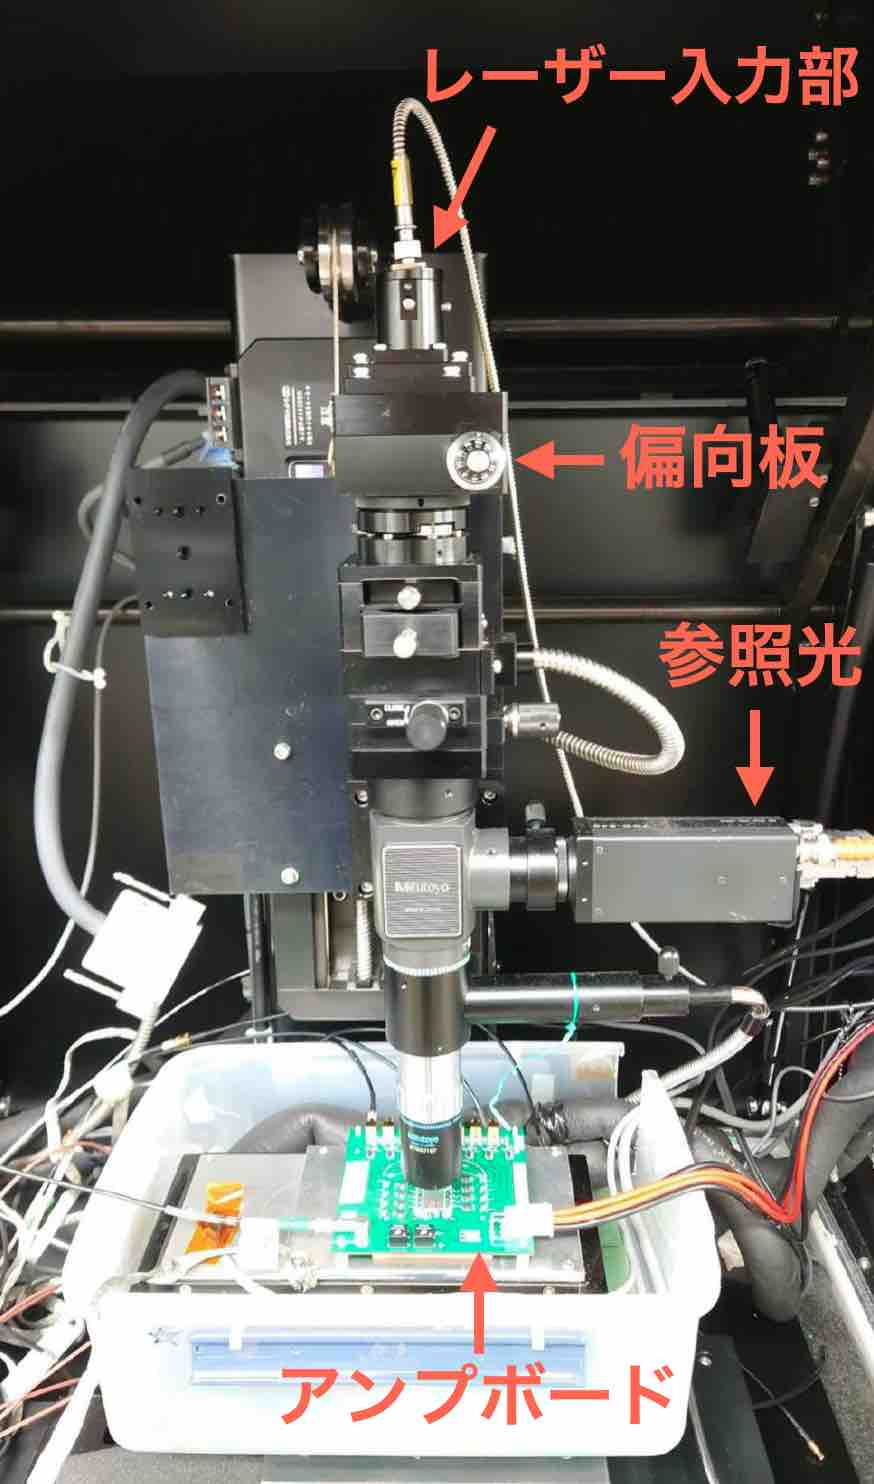
\includegraphics[width=5cm]{fig/ch4/Laser.jpg}
        \caption{赤外線パルスレーザー本体}
        \label{fg:Laser}
    \end{minipage}
    \begin{minipage}[c]{0.45\linewidth}
        \def\@captype{table}
        \tblcaption{赤外線パルスレーザーの性能表}
        \centering
        \begin{tabular}{cc}
            \hline
            モデル & KATANA 10  \\ \hline \hline
            波長 & $1064 \pm 2\:\rm{nm}$  \\ 
            パルス幅 & $35 \pm 15\:\rm{ps}$  \\ 
            平均出力 & $>10\:\rm{mW}\;\rm{at}\;1\:\rm{MHz}$  \\ 
            繰り返し周波数 & $20\:-\:80\:\rm{MHz}$  \\ 
            スペクトルバンド幅 FWHM & $<0.4\:\rm{nm}$  \\ 
            振幅ノイズ & $<4\:\%\;\rm{rms}$  (10時間)\\ 
            タイミングジッタ & $<10\:\rm{ps}$  \\ \hline
        \end{tabular}
        \label{tab:Laser_performance}
    \end{minipage}
\end{figure}

\subsection{使用するセンサーとアンプボードの接続}

今回の測定で用いる信号増幅用アンプ搭載基板(KEK16チャンネルアンプボード)が 図\ref{fg:Ampboard} で最大16チャンネルの信号を読み出すことができる。
また、アンプボードにLGAD検出器を設置した様子が 図\ref{fg:Amp_LGAD} である。
LGAD検出器とアンプボードは、ワイヤーを伝わって信号を送り出される。
今回用いたLGAD検出器は、1 chPadと呼ばれる電極が1つのAC-LGAD検出器であるため、検出器の信号は1つのチャンネルのみ出力される。
そのため、信号をアンプボードへ送るために電極からアンプボードの入力端子に1本のワイヤーで繋がっている。
アンプボードとアルミニウムが繋がっている3本のワイヤーは、高電圧をLGAD検出器に印加するためのワイヤーである。
LGAD検出器に高電圧が印加される様子を、図\ref{fg:Amp_side} に示す。この図はLGAD検出器とアンプボードを側面から見た様子である。
高電圧電源がアルミニウムから導電性テープを通ってLGAD検出器に高電圧を印加することができる。
図\ref{fg:Amp_side} の最下層にあるG10は、エポキシガラス繊維樹脂の絶縁の板であり、高電圧が外部に流れない仕組みである。
使用する高電圧電源は Tektronix 社製 Keithley2410 を使用した。また、アンプボードに電力を供給するための低電圧電源はTEXIO社のPW8-5ADPSで6 Vの電圧をかけた。
この時、電流値は0.5 Aだった。

\begin{figure}[h]
    \begin{minipage}[b]{0.5\linewidth}
        \centering
        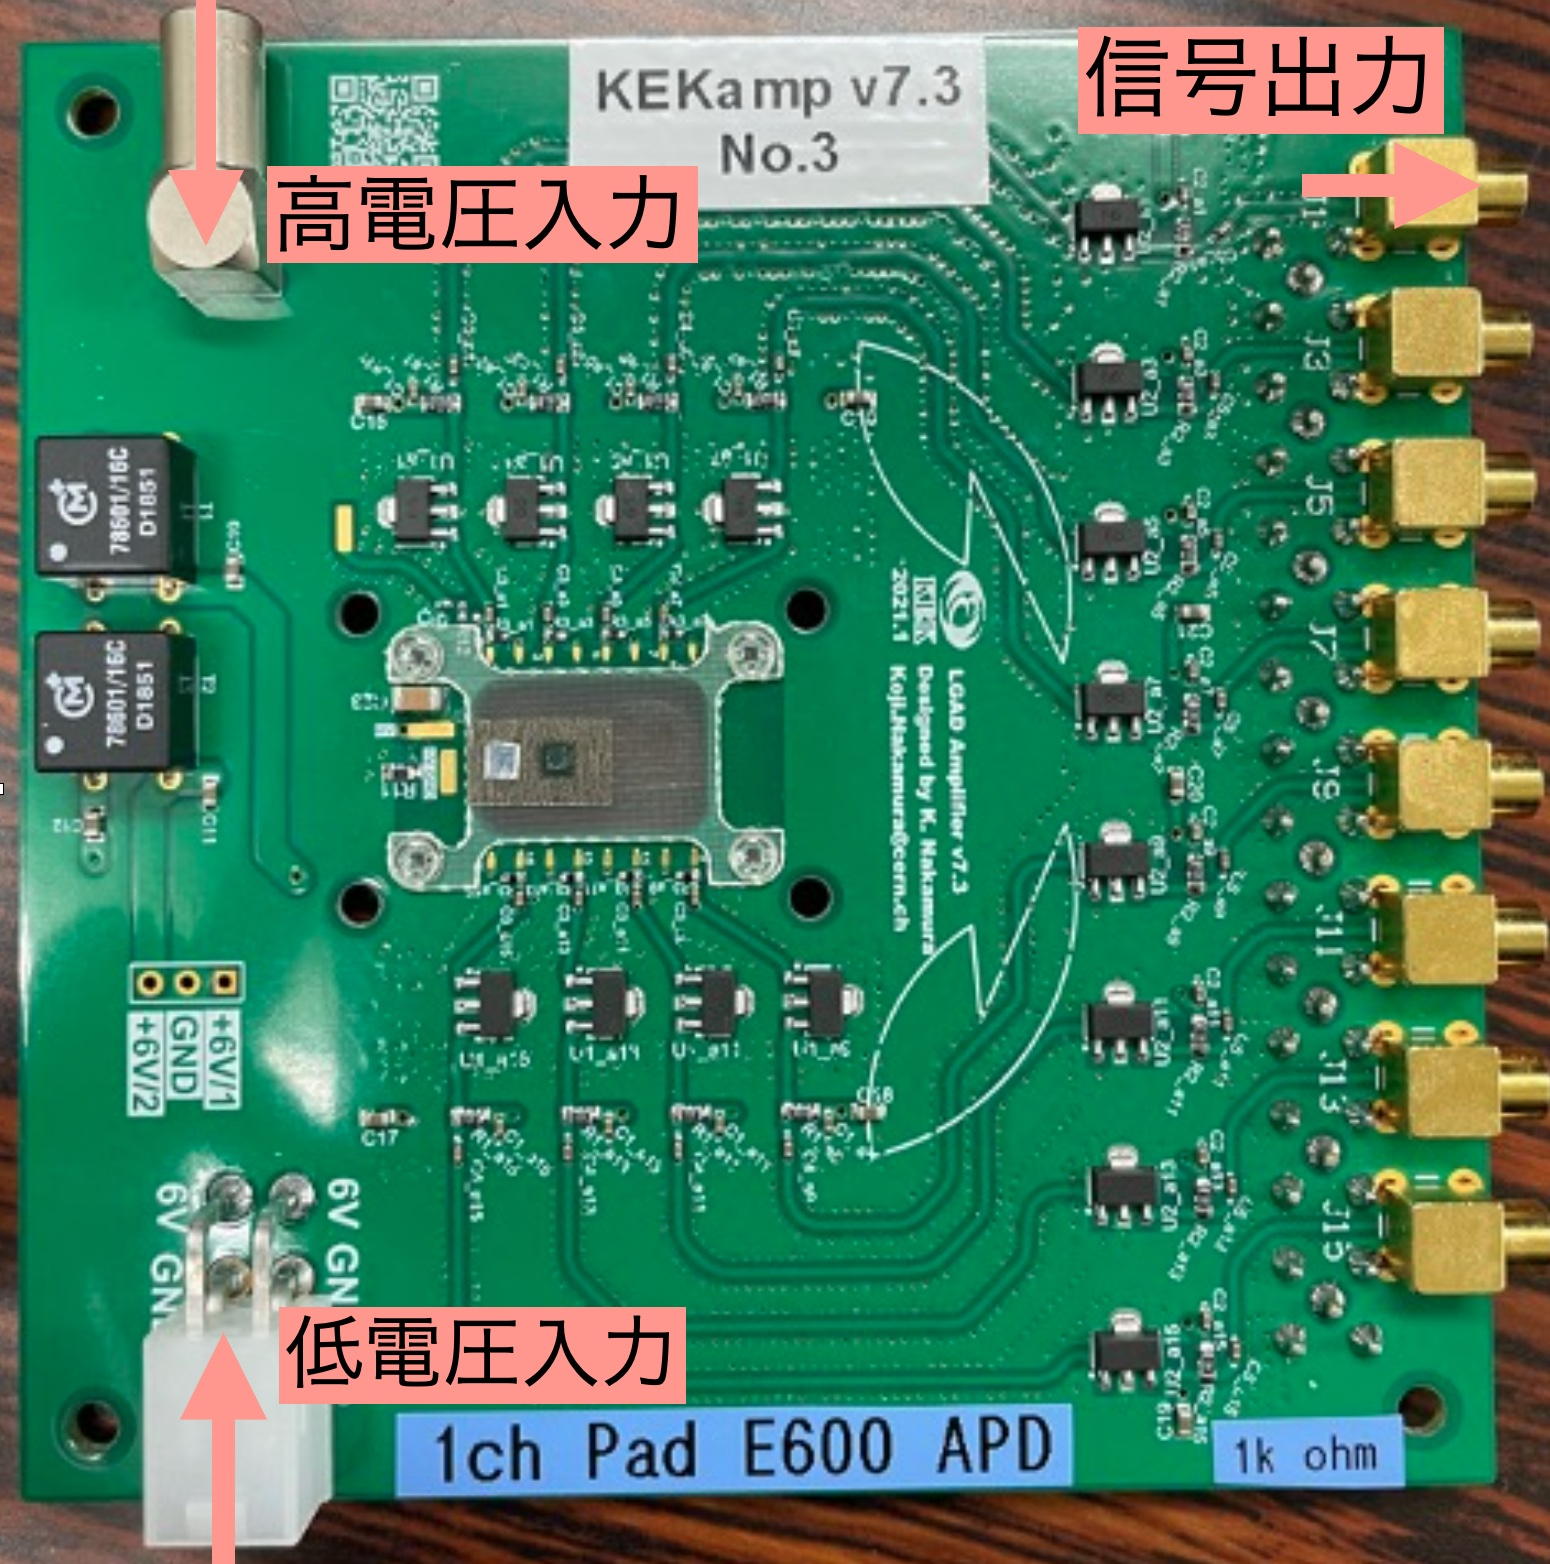
\includegraphics[width=6cm]{fig/ch4/Ampboard.jpeg}
        \caption{KEK16チャンネルアンプボード}
        \label{fg:Ampboard}
    \end{minipage}
    \begin{minipage}[b]{0.5\linewidth}
        \centering
        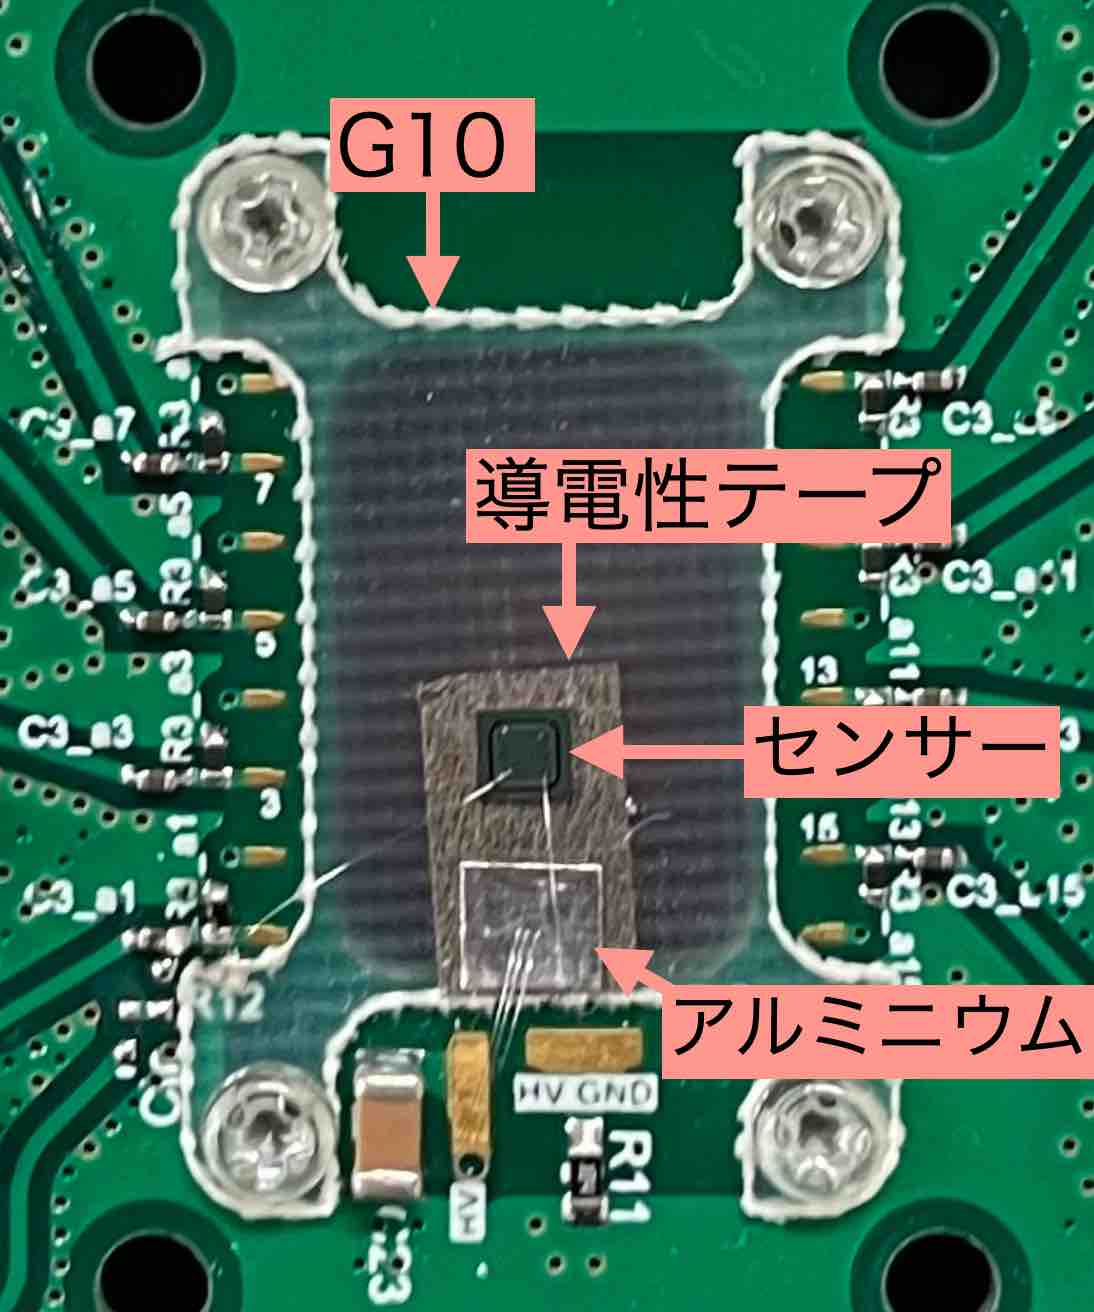
\includegraphics[width=4cm]{fig/ch4/Amp_LGAD.jpg}
        \caption{アンプボードにセンサーを設置した様子}
        \label{fg:Amp_LGAD}
    \end{minipage}
\end{figure}

\begin{figure}[h]
    \centering
    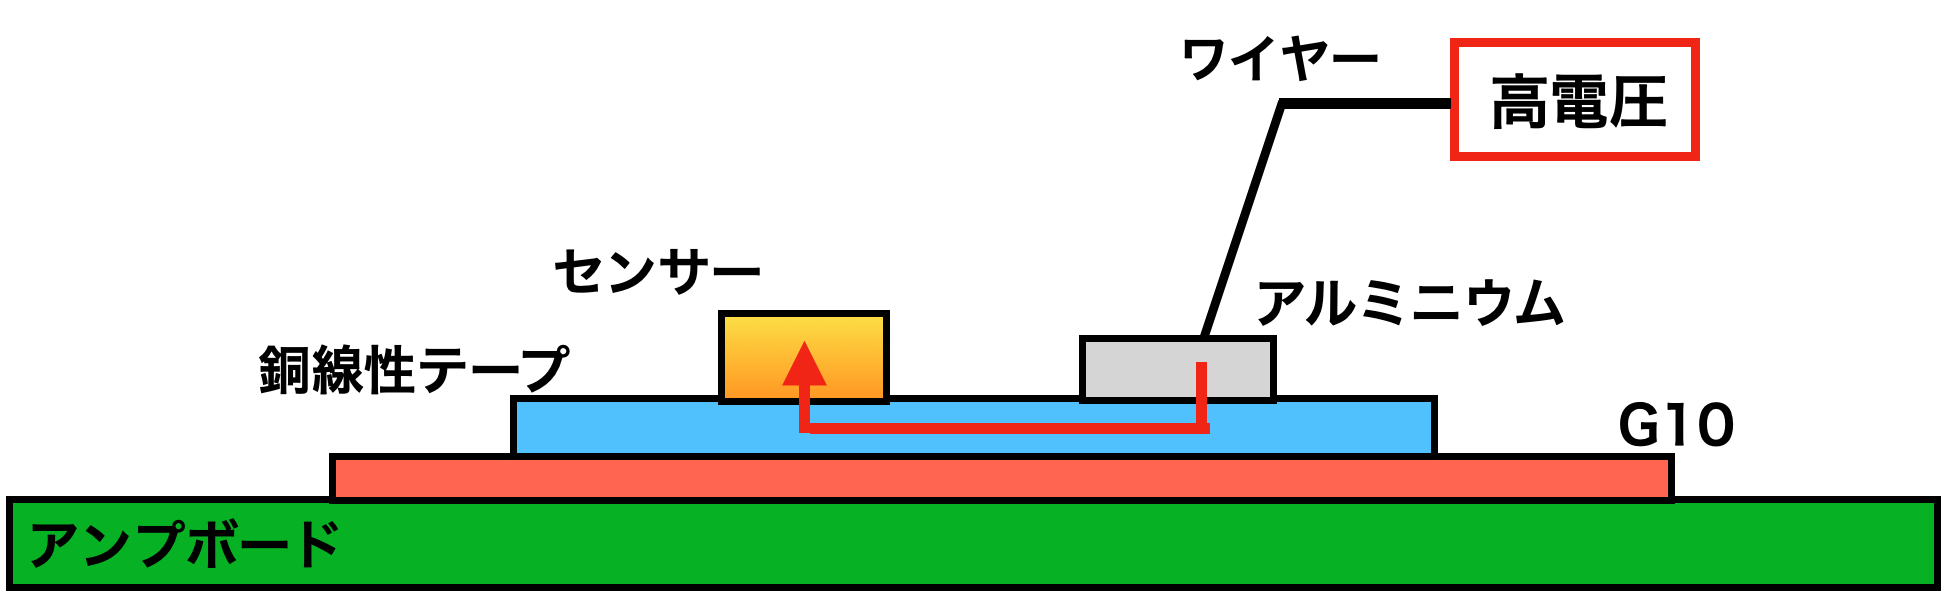
\includegraphics[width=10cm]{fig/ch4/Amp_side.png}
    \caption[センサーに高電圧を印加させる様子]{センサーに高電圧を印加させる様子\\アルミニウムから導電性テープを通ってセンサーに電圧が印加される}
    \label{fg:Amp_side}
\end{figure}

\subsection{レーザー測定のセットアップ}

以下の 図\ref{fg:Laser_setup} にこの実験の測定のセットアップを示す。
赤外線パルスレーザーをセンサーに入射し、センサーからの信号をアンプボードで増幅を行い、オシロスコープへと信号を送る。
トリガーはレーザー本体からオシロスコープへ送っている。トリガーと信号を受け取ったオシロスコープはPCへとデータを送り出す。
使用するオシロスコープは、TELEDYNE LECROY 社の WaveRunner 8000HD 8チャンネル 高分解能オシロスコープで、サンプリングレートは最大10GS/sである。
センサーとアンプボードの下には、アンプボードの発熱による温度上昇を抑えるために、
15${}^\circ$Cに設定されたチラーユニットと20${}^\circ$Cに設定されたペルチェ素子を設置した。
この装置の冷却が銅板に伝わり、空冷によってセンサーの温度上昇を抑えている。
また、センサーに光が入ると、センサーの暗電流が大きくなってしまうため、測定のセットアップを遮光するためにボックスの中に設置した。
一度の測定のイベント数は65535イベントでこのイベント数はオシロスコープの一回の測定による上限値である。

\begin{figure}[h]
    \centering
    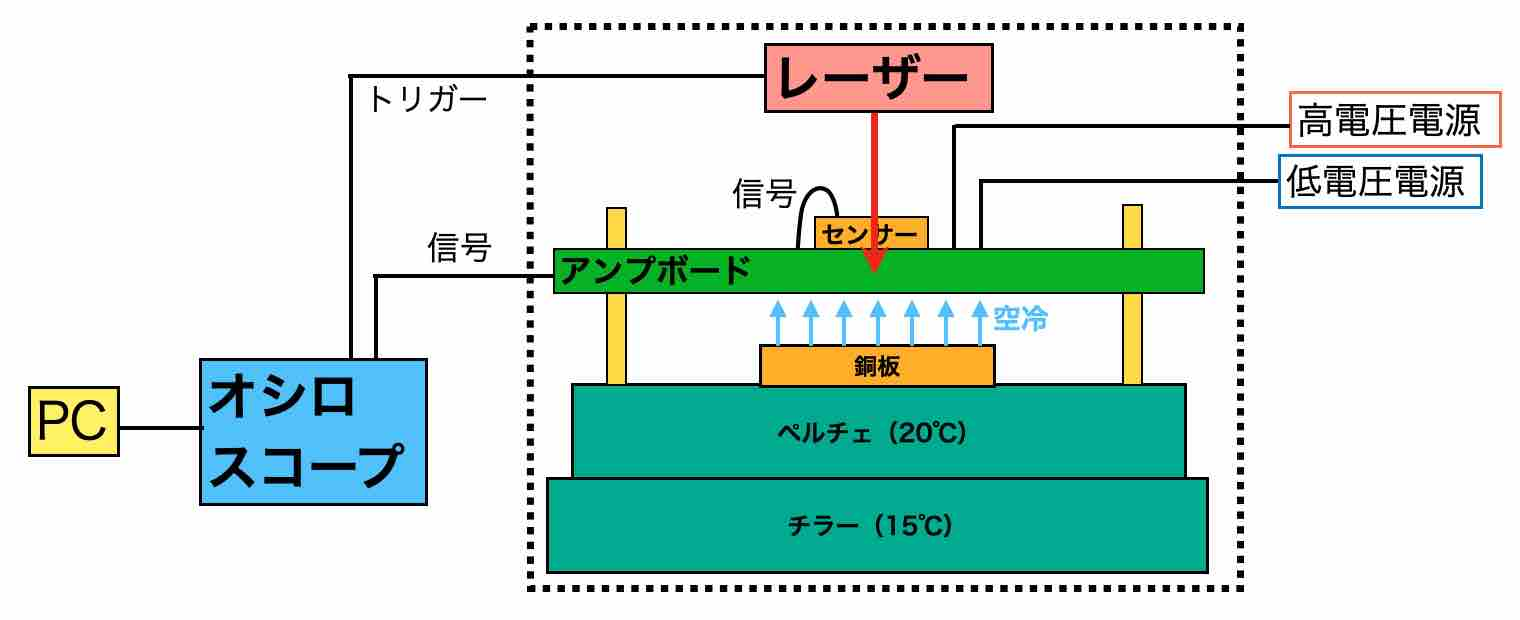
\includegraphics[width=14cm]{fig/ch4/Laser_setup.jpg}
    \caption[レーザー測定のセットアップ]{レーザー測定のセットアップ\\チラーとペルチェによってセンサーとアンプボードが空冷される。遮光ボックス(点線部)の中に測定系を設置している。レーザー本体からトリガーをアンプボードから信号をオシロスコープへ送る。}
    \label{fg:Laser_setup}
\end{figure}

レーザー光は50 倍の対物レンズを用いて、直径約 1.3 $\rm{\mu m}$に絞ることができる。
レーザーと同じ光軸上を進む参照光を用いて、レーザーがセンサーの中心に来るように調節し、焦点を合わせる。
位置と焦点の調節は、ステージコントローラを使って、0.1 $\rm{\mu m}$単位でxyz軸方向に動かすことができる。
図\ref{fg:LasertoAmp} にあるように、xy軸がビーム軸に対して垂直方向に、z軸がビーム軸と同じ方向に動かすことができる。
xy軸を動かすことでレーザー窓の中心に参照光が来るように調節でき、z軸を動かすことで、レーザーの焦点を調節することができる。

今回の測定系では低電圧をアンプボードにかけると、アンプボードの発熱によって温度膨張が生じ、図\ref{fg:Focus} のように焦点がずれてしまう。
そのため、チラーとペルチェの空冷によって、アンプボードとセンサーが熱平衡状態になってから焦点を合わせた。
光による暗電流の増加を防ぐために、測定系は遮光ボックス内に設置してある。また、測定を開始する際には、参照光を消してから測定を行った。


\begin{figure}[h]
    \begin{minipage}[b]{0.5\linewidth}
        \centering
        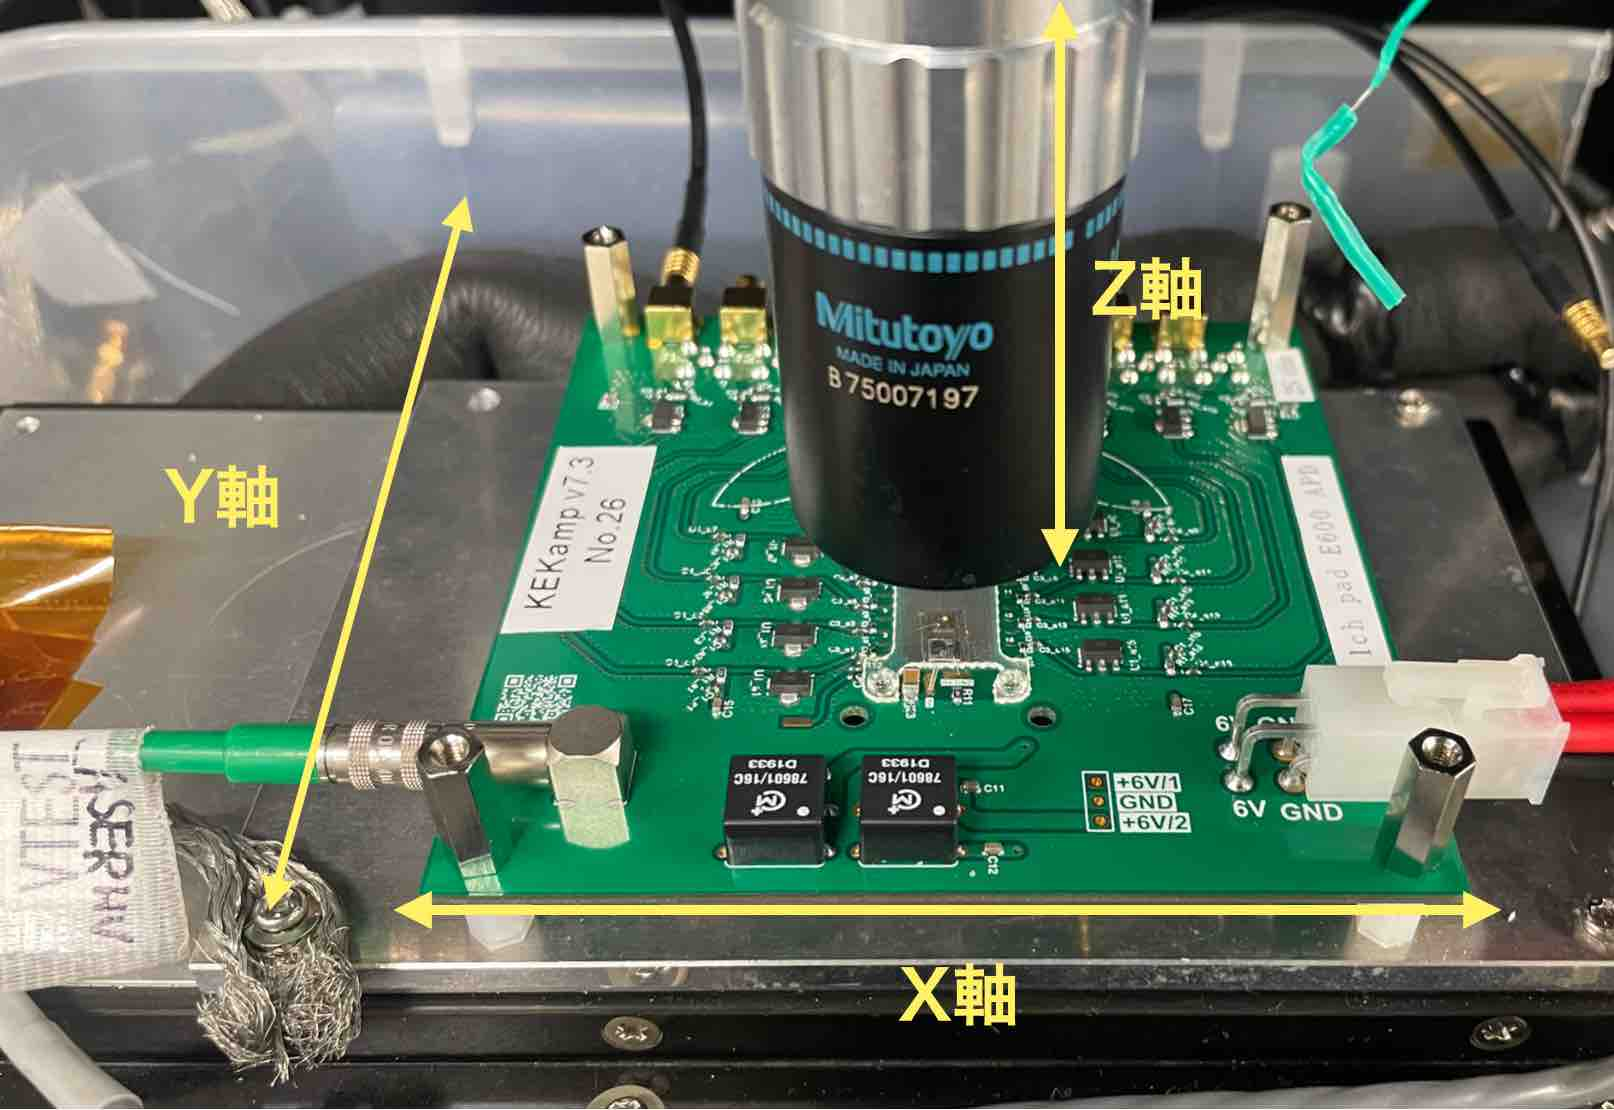
\includegraphics[width=7cm]{fig/ch4/LasertoAmp.jpg}
        \caption[レーザーの入射位置と焦点の調節]{レーザーの入射位置と焦点の調節\\xyz軸を動かして、位置と焦点を調節できる。}
        \label{fg:LasertoAmp}
    \end{minipage}
    \begin{minipage}[b]{0.5\linewidth}
        \centering
        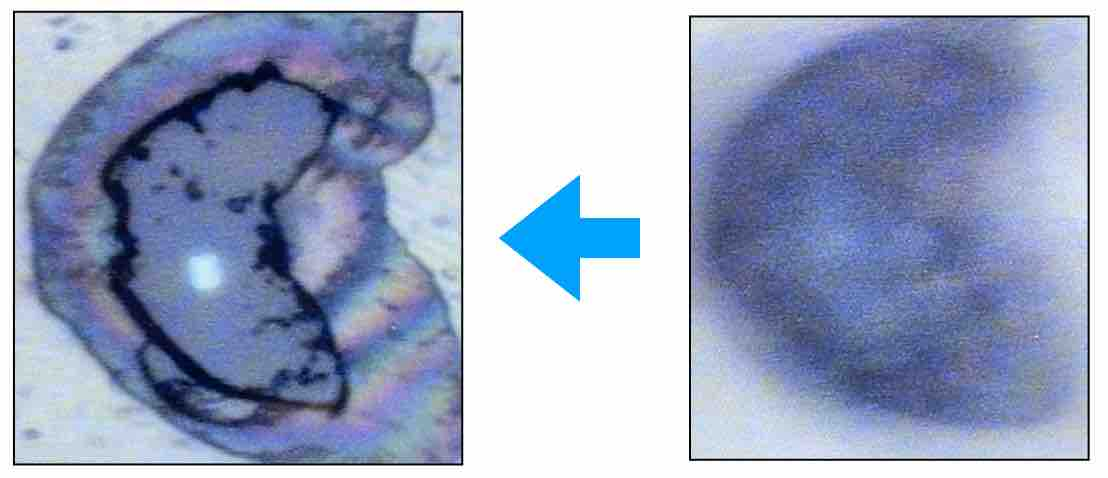
\includegraphics[width=8cm]{fig/ch4/Focus.jpg}
        \caption[レーザーの焦点の様子]{レーザーの焦点の様子\\右が焦点を合わせる前、左が焦点を合わせた後}
        \label{fg:Focus}
    \end{minipage}
\end{figure}


